
\documentclass{UoYCSproject}

\addbibresource{Report.bib}
\usepackage{enumerate}
\newcommand\independent{\protect\mathpalette{\protect\independenT}{\perp}}
\def\independenT#1#2{\mathrel{\rlap{$#1#2$}\mkern2mu{#1#2}}}
\usepackage{tikz}
\usepackage{pgflibraryarrows}
\usepackage{multirow}
\usepackage{longtable}
\usepackage[ruled,vlined]{algorithm2e}

\begin{document}
\pagenumbering{roman}
\title{Learning Causal Networks in Python}
\author{James Callan}
\supervisor{James Cussens}
\MEng
\date{}

\maketitle

\listoffigures
\listoftables

\begin{summary}
\end{summary}
\chapter{Introduction}
The aim of this report is to detail the implementation of various algorithms to learn causal networks in python.These algorithms have already been implemented in the statistical programming environment R. However, recently python has become more widely used in the field of statistical computation.\\

Python offers a number of advantages over R. Python is much more widely used in general than R so an implementation in python would be accessible to a wider array of developers.Python is also used in a variety of settings as it is a general purpose programming language. This would allow the software implementation to be integrated into many different systems, written in python, with relative ease.\\

\chapter{Literature Review}

\section{Causal Networks}

Causal Networks are graphical models which represent a set of variables, their conditional dependencies, and their causal relationships~\parencite{verma1990causal} as a Directed Acyclic Graph (DAG) or a Maximal Ancestral Graph (MAG). The nodes of the Graph represent the variables. The edges of the graph represent causality, the direction of the edge represents the direction of causality with parent nodes causing child nodes~\parencite{verma1990causal}. 

In a DAG all edges have a single direction, whereas in a MAG edges may be directed or bidirectional ~\parencite{zhang2008causal}.

\begin{figure}[h]
	\begin{center}		
	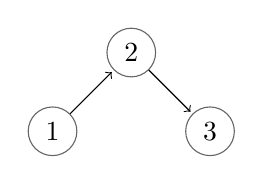
\begin{tikzpicture}[shorten >=1pt,->]
	\tikzstyle{vertex}=[circle, draw=black!60, minimum size=12pt]
	\node[vertex] (G_1) at (-1,-1) {1};
	\node[vertex] (G_2) at (0,0)   {2};
	\node[vertex] (G_3) at (1,-1)  {3};
	\draw [->] (G_1) -- (G_2);
	\draw [->] (G_2) -- (G_3);
	\end{tikzpicture}
\end{center}
\caption{A DAG with 3 nodes and 2 edges}
\end{figure}


\begin{figure}[h]
	\begin{center}	
	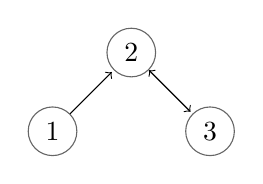
\begin{tikzpicture}[shorten >=1pt,->]
	\tikzstyle{vertex}=[circle, draw=black!60, minimum size=12pt]
	\node[vertex] (G_1) at (4,-1) {1};
	\node[vertex] (G_2) at (5,0)   {2};
	\node[vertex] (G_3) at (6,-1)  {3};
	\draw [->] (G_1) -- (G_2);
	\draw [<->] (G_2) -- (G_3);
	\end{tikzpicture}\\
\end{center}
	\caption{A PDAG with 3 nodes and 2 edges}
\end{figure}



The learning of causal networks allows relationships between variables to be uncovered and presented in a simple and human readable fashion. This can provide useful information for further data analysis as the set of variables that cause another could be used to predict it's value.

\section{Probability and Independence}
In probability theory we can quantify our confidence in a particular event $ E $ occurring. This confidence, denoted as $ p(E) $ is a real number between 1 and 0. $  p(E) = 1 $ representing a certainty and $  p(E) = 0 $ representing $E$ being impossible.

In the case of random variables an event would be a variable $X$ taking a particular value $x_i$, where $x_i$ is a member of the set $x = \{x_1, x_2, ..., x_n\}$ of possible values $X$ can take. The probability of this event is denoted as $p(X=x_i)$.

The probability distribution $p(X=x)$ or simply $p(X)$ defines the probabilities for every value which $X$ can take. 

Distributions of more than one variable can be described with joint distributions. For Variables $X$ and $Y$ the distribution $p(X,Y)$  describes the probability of both $X$ and $Y$ taking particular values simultaneously. 

Joint distributions can also describe how the value of one variable can effect the value of an other. $p(X|Y)$ describes the probabilities of $X$ taking particular values ''given'' a value that $Y$ has taken. $p(X|Y)$ is defined as $p(X,Y)/p(Y)$.

If two variables are independent there is no correlation between the values they take. That is for two variables $X$ and $Y$, the distribution $p(X|Y)$ would be the same for all values of $Y$. Therefore $p(X|Y) = p(X)$. If two variables are independent we can determine that there is no causal relationship between them.

Given the definition $p(X|Y) = p(X,Y)/p(Y)$ and $p(X|Y) = p(X)$ when $X$ and $Y$ are independent, it easy to see that $p(X,Y) = p(X)p(Y) $ if $X$ and $Y$ are independent.

Two variables $X$ and $Y$ can be considered independent conditioned on a third variable $Z$ if there is no correlation between $X$ and $Y$ for given the value of $Z$.

In this case $p(X|Y,Z) = p(X|Z)$, as the value of $Y$ has no impact on the value of $X$. The definition of conditional distributions shows $p(X|Y,Z) = \frac{p(X,Y,Z)}{p(Y,Z)}$, and $p(Y,Z) = p(Y|Z)P(Z)$. Using theses definitions and basic algebra $p(X,Y|Z) = p(X|Z)p(Y|Z)$ can be shown when $X$ and $Y$ are conditionally independent on $Z$.

\section{D Separation}

A path is any sequence of adjacent edges regardless of their directionality. A collider is node in a path which is both entered and left on edges which are directed toward the node. Unblocked refers to a path that does not traverse a collider~\parencite{pearl2003causality}.
\begin{figure}[h]
\begin{center}
	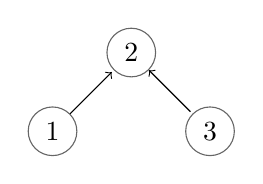
\begin{tikzpicture}[shorten >=1pt,->]
	\tikzstyle{vertex}=[circle, draw=black!60, minimum size=12pt]
	\node[vertex] (G_1) at (-1,-1) {1};
	\node[vertex] (G_2) at (0,0)   {2};
	\node[vertex] (G_3) at (1,-1)  {3};
	\draw [->] (G_1) -- (G_2);
	\draw [<-] (G_2) -- (G_3);
	\end{tikzpicture}
\end{center}
\caption{A graph containing a collider}
\end{figure}

	


If every path between nodes $ X $ and $ Y $ traverses a collider, nodes $ X $ and $ Y $ are unconditionally d-separated or d-separated conditioned on the empty set ~\parencite{pearl2003causality}. Two unconditionally d-separated nodes in a causal network are considered to be independent~\parencite{pearl2009}.
\begin{figure}[h]
\begin{center}
	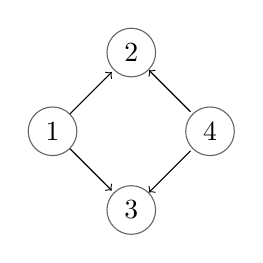
\begin{tikzpicture}[shorten >=1pt,->]
	\tikzstyle{vertex}=[circle, draw=black!60, minimum size=12pt]
	\node[vertex] (G_1) at (-1,-1) {1};
	\node[vertex] (G_2) at (0,0)   {2};
	\node[vertex] (G_3) at (0,-2)  {3};
	\node[vertex] (G_4) at (1,-1)  {4};
	\draw [->] (G_1) -- (G_2);
	\draw [<-] (G_2) -- (G_4);
	\draw [->] (G_1) -- (G_3);
	\draw [<-] (G_3) -- (G_4);
	\end{tikzpicture}
\end{center}
\caption{A DAG in which nodes 1 and 4 are D-Separated}
\end{figure}

\begin{figure}[h]
\begin{center}
	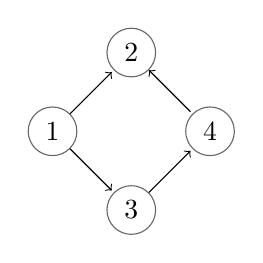
\begin{tikzpicture}[shorten >=1pt,->]
	\tikzstyle{vertex}=[circle, draw=black!60, minimum size=12pt]
	\node[vertex] (G_1) at (4,-1) {1};
	\node[vertex] (G_2) at (5,0)   {2};
	\node[vertex] (G_3) at (5,-2)  {3};
	\node[vertex] (G_4) at (6,-1)  {4};
	\draw [->] (G_1) -- (G_2);
	\draw [<-] (G_2) -- (G_4);
	\draw [->] (G_1) -- (G_3);
	\draw [->] (G_3) -- (G_4);
	\end{tikzpicture}
\end{center}

\caption{A DAG in which nodes 1 and 4 are not D-Separated}
\end{figure}


Two nodes X and Y are d-separated conditioned on set Z if:
\begin{enumerate}
	\item There exists no unblocked path from $ X $ to $ Y $ that does not traverse any members of $ Z $.~\parencite{pearl2003causality}
	\item There is no blocked path from $ X $ to Y in which all colliders are members of $ Z $ or have descendants in $ Z $. ~\parencite{pearl2003causality}
\end{enumerate} 

Causal networks represent conditional independence with d-separation, variables X and Y are conditionally independent on set Z if nodes X and Y are d-separated conditioned on nodes in set Z~\parencite{verma1990causal}.

\section{Faithfulness}


By testing for d-separation of variables X and Y given conditioning set Z on a graph we can see if $X \independent Y | Z$ ~\parencite{pearl2009}. However, the reverse is only true if the distribution is faithful to the graph. That is, if a distribution is faithful to a graph then all independence relationships are represented on the graph and only these relationships are present ~\parencite{scheines1997introduction}. Assuming faithfulness allows the topology of a graph to be learned by testing pairs of variables for independence given various conditioning sets.

\section{Discriminating paths}
For the FCI and RFCI algorithms the notion of discriminating paths is needed. A path $\pi$ = (A, .., X,Y,Z) is discriminating a discriminating path for Y if:

\begin{enumerate}
	\item $\pi$ must include at least 3 edges
	\item Y is a non-endpoint on $\pi$ and is adjacent to Z on $\pi$.
	\item A is not adjacent to Z and every other node is a collider on $\pi$ and a parent of Z. ~\parencite{colombo2012learning} 
\end{enumerate}

\begin{figure}[h]
\begin{center}
	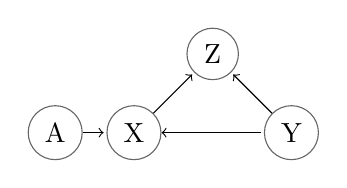
\begin{tikzpicture}[shorten >=1pt,->]
	\tikzstyle{vertex}=[circle, draw=black!60, minimum size=12pt]
	\node[vertex] (G_1) at (0,0) {A};
	\node[vertex] (G_2) at (1,0)   {X};
	\node[vertex] (G_3) at (3,0)  {Y};
	\node[vertex] (G_4) at (2,1)  {Z};
	\draw [->] (G_1) -- (G_2);
	\draw [<-] (G_2) -- (G_3);
	\draw [->] (G_2) -- (G_4);
	\draw [->] (G_3) -- (G_4);
	\end{tikzpicture}
\end{center}


\caption{$A-X-Y-Z$ is a discriminating path on $ Y $}
\end{figure}

\section{Possible D-Separation Set}
The FCI algorithm must also find the possible-d-separation set for every node on the graph. This set consists of all nodes which could be d-separated based on some conditioning set. For a particular node (X) in a graph this set consists of all nodes (Y) for which there exists a path from X to Y for which every triple (A,B,C) is a triangle or the node B in the triple is a collider on the path.

\section{Tests for Independence}
When trying to find causal relations between variables tests for independence and conditional independence must be performed. These tests allow us to find correlation between variables and also find out if the correlation between two variables is actually caused by another.

One such test is the $\chi^2$ test, this test gives the probability that some data was drawn from a particular distribution.

If the variables $X$ and $Y$ are independent then $p(X,Y) = p(X)p(Y)$. Both of these distributions can be calculated from data. The $\chi^2$ test can then be used to find the probability that they are equal.

To estimate $p(X,Y)$ the counts of all pairs of values taken by the variables can be found. They can then divided by the count of all data points. These counts can be stored in a table with the values of $X$ as columns, values of $Y$ as rows (or visa versa) and entries as observed counts, for ease of access. This type of table is known as a contingency table.

\begin{table}[h!]
	\centering
	\begin{tabular}{c|c c c c c c c}
		X & 1 & 1 & 0 & 1 & 0 & 1 & 1\\ \hline
		Y & 0 & 1 & 1 & 1 & 0 & 1 & 0\\
	\end{tabular}
\\
	\begin{tabular}{c|c|cc|}
		\multicolumn{2}{c}{}& \multicolumn{2}{c}{X} \\ \cline{3-4}
		\multicolumn{2}{c|}{} & 0 & 1 \\ \cline{2-4}
		\multirow{2}{*}{Y} & 0 & 1 & 2\\
		& 1 & 1 & 3 \\
		\cline{2-4} 
	\end{tabular}
\caption{Example Contingency Table For Two Variables}
\end{table}

To estimate the distribution $p(X)$, the count of points in which $X$ takes a value over the total number of points for all values of $X$. The counts can be found with the sum of the columns of the contingency table. The same can be done for $p(Y)$ with the rows of the table.\\

The $\chi^2$ statistic can then be calculated with:

\begin{center}
	$\chi^2 = \sum\frac{(p(X)p(Y)-p(X,Y))^2}{p(X)p(Y)}$
\end{center}

The $\chi^2$ value can then be passed to a cumulative density function and a p-value returned. The function used is dependent upon the degrees of freedom. The degrees of freedom are equal to the $(no. rows -1)*(no. columns -1)$. The p-value represents how likely it is that the two variables are independent.\\

The test is similar for conditional independence. The $chi^2$ statistic now depends on conditional distributions. If $X \independent Y | Z$ $p(X,Y|Z) = p(X|Z)p(Y|Z)$. Therefore:\\

\begin{center}
	$\chi^2 = \sum\frac{(p(X|Z)p(Y|Z)-p(X,Y|Z))^2}{p(X|Z)p(Y|Z)}$
\end{center}

These values can all be found by calculating a contingency table for $X,Y $ and $ Z$.\\

This statistic can then be used in the same way as before to calculate a p-value. However, the degrees of freedom are multiplied by the possible values of $Z -1$. 

\subsection{Algorithms For Learning Causal Networks}
\subsection{Constraint Based Methods}
There have been a number of algorithms developed to learn graphical causal representations from data. Over the course of this project, I plan to implement: The PC algorithm ~\parencite{spirtes1991algorithm}, the Fast Causal Inference (FCI) algorithm ~\parencite{colombo2012learning}, and the Really Fast Causal Inference (RFCI) Algorithm ~\parencite{colombo2012learning}.

Rather than learning an individual DAG the PC algorithm learns a set of DAGs which could represent the causal relationships found in the data. In cases where the direction of an edge is unclear no direction is specified. The output of the algorithm is a partially directed acyclic graph which represents the set DAGs with all possible orientations of undirected edges~\parencite{spirtes1991algorithm}.

The FCI and RFCI algorithms learn partial ancestral graphs (PAGs) which represent the set of MAGs that fit the data ~\parencite{colombo2012learning}. Unlike in the PC algorithm if the direction of an edge can not be determined it is assumed that there is some set of latent variables influencing the nodes being tested. Each end of an edge can be one of three things in a PAG, an arrow in every MAG ($>$), a tail in every MAG ($-$) or an arrow in at least one MAG and a tail in at least one MAG ($o$), ends of an edge denoted by $*$ can be any of the specified types. This allows for a richer display of information than a partial DAG~\parencite{colombo2012learning}.

The PAG generated by the FCI algorithm is considered to be less accurate than the PAG generated by the RFCI algorithm. This is because the FCI algorithm performs more tests than the RFCI algorithm. These tests give us more confidence in the presence and the orientation of edges however this comes at the cost of speed.
\subsection{Score Based Methods}
The above algorithms are all constraint based. There is another class of algorithm which are score based. Rather than finding graphs using the rules that define the networks, score based methods generate random graphs and assign them a score based on how well they fit data.\\

An example of a scored based method is the graphical lasso algorithm. 

\section{Computing a skeleton}
All three algorithms begin by calculating the skeleton of the graph. The skeleton consists of the edges that are present in the partial DAG or PAG however all edges are undirected. The separation set of two variables ($sepSet(x,y)$) contains the smallest set of variables that the pair are conditionally independent on.  When calculating the skeleton the separation set of each pair of variables is also recorded as it is needed to orient the edges of the graph~\parencite{colombo2012learning, spirtes1991algorithm}.

The skeleton is calculated using a series of conditional independence tests. These conditional independence tests are dependent on the type of input data, therefore conditional independence tests can be defined independently of the algorithm. The conditional independence tests must be able to determine if two variables are indpendent based on some set of other variables from data.

To begin the skeleton computation the fully connected undirected graph of all variables is constructed and then conditional independence tests are performed to determine which edges to remove.

Adjacent pairs of variables are tested for independence conditioned upon set of variables adjacent to them. The size of these sets starts at 0 but is incremented after all adjacent pairs have been tested. This repeats until there are not enough adjacent variables to fill the conditioning set.\\

The edges which have not been removed form the skeleton of the graph which is needed for the PC, FCI and RFCI algorithms along with the recorded separation sets of removed edges ~\parencite{spirtes1991algorithm}.


\begin{algorithm}[H]
	\DontPrintSemicolon

	\KwIn{Data, Independence Test}
	\KwResult{Estimated Skeleton, Separating Set of each Variable}
	\Begin{
	$k = 0$\;
	$N =$ list of variables which make up the data\;
	$G= $ fully connected undirected graph with nodes N\;
	\While{There is some $S \subseteq  adj(X,G) \setminus Y$ and $|S| = k$ for some $X \in N, Y \in adj(X,G) $}{
		\For{$X \in N$}{
			\For{$Y \in adj(X,G)$}{
				\For{$S \subseteq adj(X,G)\setminus Y$ where $|S| = k$}{
					\If{$X \independent Y | S$}{
						remove edge $X-Y$ from G\;
						$Sepset(X,Y) = S$\;
						$Sepset(Y,X) = S$\;
					}
				}
				
			}
		}
	$k += 1$\;
	}
}
\caption{Algorithm to Estimate Skeleton of Causal Network}
\end{algorithm}
\section{The PC Algorithm}
After generating the skeleton and separation sets of pairs of nodes, the pc algorithm attempts to orient the undirected edges of the graph.

It begins by searching for colliders. For each triple of vertices A, B, and C where A and B are adjacent, B and C are adjacent, but A and C are not adjacent orient the edges A-B-C to A$\rightarrow$B$\leftarrow$C if B is not in the separation set of the pair (A,C).

Once colliders are specified other edges can be oriented. This is done by repeating two steps until no more edges can be given a direction. The algorithm for edge orientation is described in.\\


\begin{algorithm}[H]
	\DontPrintSemicolon
	
	\KwIn{Skeleton of Causal Network, Separation sets of variables}
	\KwResult{Partial Directed Acyclic Graph}
	\Begin{
	$ 	G = $ Skeleton\;
	$ 	N = $ nodes of G\;
	\For{$i,j,k \in N$}{
	\If{$k \notin adj(i,G)$ and $ j \notin sepSet(i,k)$}{
	orient $i-j-k$ as $i \rightarrow j \leftarrow k$\;
	}	
	}
	\While{No more edges can be oriented}{
	\For{$i,j,k \in N$}{
	\If{ $ k \notin adj(i,G)$}{
	orient $ i\rightarrow j-k $ as $ i\rightarrow j \rightarrow k $\;
	}
	\If{There is a directed path from $i$ to $j$ in $G$}{
	orient $ i-j $ as $ i\rightarrow j$\;
	}
	}
	}
	}
	
	\caption{PC Algorithm to Orient Edges}
\end{algorithm}

\section{The FCI algorithm}

The FCI algorithm starts in the same way as the PC algorithm using exactly the process of conditional independence tests to estimate a skeleton of the final graph. It also orients colliders in the same way, producing a PDAG.

Next, the final skeleton of the graph is obtained from the PDAG G. To do this The possible d-separators of every variable must be found in G. For variable X, the possible d separators set in nG ($PossibleDSep(X,G)$) consists of all variables Y for which there is some path $\pi = path(X,Y)$ in G, such that in every sub path $A,B,C$, $B$ is a collider or $A,B,C$ form a triangle. All adjacent variables ($X,Y$) are the tested for conditional independence, conditioned on every subset of each of the possible d separators set. If the test finds conditional independence the edge $X,Y$ is removed and the conditioning set recorded as a separation set. 

The PDAG can then be converted to a PAG by setting all edges to $o-o$.

Next the colliders must be reoriented. This is done on a similar way however now edges can be bi-directional.

Once the final skeleton has been estimated, A series of orientation rules can be performed repeatedly until no more orientations can be found. Theses rules where originally described in. However these rules did not fully orient the $-$ tags of the graph ~\parencite{ZHANG20081873}. 10 rules were found in ~\parencite{ZHANG20081873} which allow full orientation of the graph. The complete set of rules is used in the R implementation and will also be used in the python implementation.


\begin{algorithm}[H]
	\DontPrintSemicolon
	
	\KwIn{Skeleton of Causal Network, Separation sets of variables}
	\KwResult{Partial Ancestral Graph}
	\Begin{
		$ 	G = $ Skeleton\;
		$ 	N = $ nodes of $G$\;
		Set all edges of $G$ to $\circ-\circ$\;
		\For{$i,j,k \in N$}{
			\If{$k \notin adj(i,G)$ and $ j \notin sepSet(i,k)$}{
				orient $i *-\circ j \circ-* k$ as $i \circ\rightarrow j \leftarrow \circ k$\;
			}	
		}	
		\For{$i \in N$}{
			\For{$j \in adj(i,G)$}{
				\For{$T \subseteq PossibleDSeps(i,G) \ i$}{
					\If{$i \independent j| T$}{
						remove edge $i*-*j$ from $G$\;
						$sepSet(i,j) = T$\;
						$sepSet(j,i) = T$\;
					}
				}	
			}
		}
		Set all edges of $G$ to $\circ-\circ$\;
		\For{$i,j,k \in N$}{
			\If{$k \notin adj(i,G)$ and $ j \notin sepSet(i,k)$}{
				orient $i *-\circ j \circ-* k$ as $i \circ\rightarrow j \leftarrow \circ k$\;
			}	
		}
		\While{No more edges can be oriented}{
			Apply $R1-R10$ from ~\parencite{ZHANG20081873}
		}
	}
	
	\caption{FCI Algorithm to Orient Edges}
\end{algorithm}


\section{RFCI Algorithm}
Like the other two algorithms the RFCI begins by estimating the skeleton of the final graph.

Next the colliders in the graph are found, this is done differently than in the two previous algorithms. We created and empty list L and for each triple (A,B,C) in the list of unshielded triples we check if both:

\begin{enumerate}[i]
	\item $A \independent$ $B$ $|$ $((sepset(A,B) \setminus \{C\}))$
	\item $B \independent$ $C$ $|$ $((sepset(A,B) \setminus \{C\}))$
\end{enumerate}

where sepset(X,Y) is the separating set of Nodes X and Y. If both of these tests hold, add to list L. If only the first test holds, find the minimal separating set of A and B and record it as the separating set of A and B. Next, remove the edge A-B, add any newly create unshielded triples to M, and remove any destroyed triples from L and M. If only the second test passes do the same as above but for nodes B and C.

Finally the edges must be oriented. To begin edge orientation apply rules $R1-R3$ found in ~\parencite{ZHANG20081873}. Next triangles (X,Y,Z) must be found with edges $Yo-*Z$, $X<-*Y$, and $X-->Z$. Once a triangle is found the shortest discriminating path from X to Z must be found.

If a path $\pi$ exists take each pair of adjacent variables A and B on $\pi$ and creator a counter $l = 0$. Next find  a subset Y  $\subseteq (sepset(X,Y) \setminus \{A,B\})$ where $|Y| = l$. Then if $A \independent B | Y \cup S$ let sepset(A,B) = Y, delete the edge $A*-*B$ from the graph and update newly formed unshielded triples orientation using the collider orientation described earlier. If the conditional independence test fails increment $l$ and try again, testing with all subsets Y of size $l$, repeat this process until no set Y exists where |Y| = $l$ or the edge $A*-*B$ is removed. 

If no edges are removed from $\pi$ by the above process then either: orient $Yo-*Z$ as $Y-->Z$ if Y is in the sperating set of X and Z or orient $X<-*Yo-*Z$ as $X<->Y<->Z$ if not.

Finally orient as many edges using rules $R5-R10$ from ~\parencite{ZHANG20081873}.

This whole process must be repeated until it no longer alters any orientations.~\parencite{colombo2012learning}

\begin{algorithm}
	\DontPrintSemicolon
	
	\KwIn{Skeleton of Causal Network, Separation sets of variables}
	\KwResult{Partial Ancestral Graph}
	\Begin{
		$ 	G = $ Skeleton\;
		$ 	N = $ nodes of $G$\;
		$ 	L = $ empty list\;
		$ 	M = $ list of unshielded triples\;
		\While{$M$ is non-empty}{
			choose $\langle i,j,k \rangle$ from $M$\; 
			$T = sepSet(i,k) \ j$\;
			\If{$i \independent j | T$ and $k \independent j | T$}{
				add $\langle i,j,k \rangle$ to $L$
			}
			\Else{
				\For{$r \in {i,j}$}{
					\If{$r \independent j | T$ }{
						Find the minimal seperating set $Y \subseteq T$ for $r$ and $j$;
						$sepSet(r,j) = Y$\;
						$sepSet(j,r) = Y$\;
						add all triples $\langle r,*,j \rangle$ to $M$\;
						Remove all triples containing $r$ and $j$ and either $r$ or $j$ in the middle from $M$ and $L$\;
						Remove $r*-*j$ from $G$\;}
					}
				}
			Remove $\langle i,j,k \rangle$ from $G$\;
			}
			\For{ $\langle i,j,k \rangle \in L$ }{
				\If{$j \notin sepSet(i,k)$}{
					Orient $x*-\circ j \circ - * k$ as $x*-\rightarrow j \leftarrow - * k$}}
		}
	\caption{RFCI Algorithm to Orient V-Structures}
\end{algorithm}

\chapter{Design}

\section{Methodology}
When Designing software there are a number of approaches that can be taken. Most of these approaches break development down into a number of different phases and describe the order in which they should be completed.\\

Most methodologies were designed for teams of engineers, as this project was completed by one individual many components of the methodologies are redundant. However there are some principles and techniques which can be utilised by an individual developer and aid in organisation of a project.

\subsection{Waterfall}
The waterfall methodology is a linear approach to development. Each stage of development is completed all at once for the whole piece of software. This means that once a stage is completed there is no need to return to it and the development process flows in one direction like a a waterfall.

The waterfall approach is good because the whole project is rigorously planned and documented before coding begins. This allows major difficulties in projects to be dealt with before significant time has been invested. It also allows projects to be easily passed between developers as a new developer can look at the plan of the project. In less linear approaches there may be plans for future parts of software which are never documented.

The downfall of the waterfall approach comes when a project is not fixed or there is a a change in requirements, there is no stage in which plans can be modified as that would involve going backwards in development.


\subsection{Agile}
The agile approach is a methodology which focuses on iterative development. Deliverables are identified and designed individually, there is also a much greater focus on executable code than documentation than in waterfall.

Many parts of the agile methodology are not needed in this project such the parts that deal with the customer and cooperation between developers as this is a solo project without a customer.

The most important part of agile is its ability to deal with changing scope through process. Also since testing is done at each stage it will allow the project to be easily shortened or extended based on time constraints, as after every sprint a working piece of software has been developed.

\subsection{Spiral}
The spiral model for software development is a risk driven process. The spiral method can contain aspects from the other processes.

The actions taken and the amount of work done on areas of the project are determined by what would minimize risk.

Risk can be a number of things. In an industrial setting risk could be how how spending more time on a product and delaying it's release would affect it's sales figures. In a team project, risks could  consist of members of the team being unable to work on software unexpectedly because of illness. In essence, risk is anything that would be detrimental to the stakeholders in the project.

Spiral development also requires risks to be assessed at every stage of development. This would increase the work load specifically in agile as risks would need to be identified at every iteration. This would lead to a lot of repeated work that could be better spent on development or testing.  
\subsection{Chosen Approach}

The chosen approach for this project was agile. The reduced amount of documentation will speed up development. Agile development also allows the scope of the project to change over time. This allowed the scope of the project to start off small and increase if time allowed it.

For example, once the PC algorithm had been implemented, if time allowed, the project could easily be extended to include the FCI algorithm.

The spiral approach will not be used for this project as it will lead to an unnecessary increase in work for a relatively low risk project. The project also has a fairly logical order of implementation so using risk minimization to determine what to implement will not be necessary.

Within the Agile methodology there are a number of popular frameworks. However, these teams are designed for teams of software engineers with clients. Since this is a solo project without a client many parts of these frameworks will not be applicable. Therefore, the applicable parts of various frameworks were chosen and compiled into a framework that will work for this project.


\section{Requirements}
Requirements were elicited at the beginning of a sprint. A deliverable was chosen and the requirements were found for that deliverable. Requirements were found by considering how the software would be used.

\subsection{Epics}
Epics describe a very high level interaction between a user and the software. They describe the general functionality of a deliverable without discussing it's implementation. Epics were the first stage of requirement elicitation as they they capture the functionality that the requirements must capture.
\subsection{User Stories}
Each epic is then broken down into user stories. The stories describe what a user must be able to do with the software during the epic. They are fairly low level and form a set of required functionality of the software.

Users stories can be used as requirements as software that would allow user stories to occur would be functional.

\section{Sprints}
Sprints are sections of development defined by deliverables. They outline the tasks required to be completed to develop a deliverable and the time frame needed.

When a sprint is completed, the scope of the project and the requirements can be updated and modified if needed.

for this project there were four main deliverables implemented and four sprints to implement them.\\

The first sprint consisted of implementing the $\chi ^2$ conditional independence test. This test was needed before anything else could be properly implemented.

Next, the skeleton learning software was written. The skeleton is needed for all algorithms in this project so is the next logical step from the independence test.

Then the pc algorithm was fully implemented, this algorithm was the simplest of the 3 so made sense to start with. Starting with the easiest algorithm gave me experience using networkx and the other libraries being used that would be very useful in the final sprint.

Finally, the FCI algorithm was implemented. This was more complex than the pc algorithm, however the experience with the library in previous sprints greatly helped with the more complex orientation.

\subsection{Tasks}
From the stories can be formed. Theses tasks describe the software that must be implemented to fulfil the requirements.

Each sprint had a number of associated tasks. The tasks were small and each task could be verified through testing.

Each task has associated stories so that all software can be traced back to an epic. Tracing back to an epic shows that each task will in some way contribute to functional software.\\
\section{Architecture}
Only the architecture for a particular deliverable was designed in each sprint. This meant that the architecture grew over time. Considerations for general extensibility of the software needed to be made in the design phase to ease design and implementation during later sprints.\\

A class diagram was produced, this specified the relationships between classes and the functionality of each class. This diagram evolved throughout the project as various sprints were completed.\\

The class diagram for this software was fairly straightforward. This is because the software did not implement a complex system. Only a few classes were needed as most of the complexity is contained in the methods of the classes.

\subsection{Unit Testing}
Test driven development (TDD) was one of the main features of the development framework. In this development, tests were created before the actual software was written. This ensured that all software that was written would be functional. It also ensures that any refactoring performed would not compromise the functionality of software.

All software was tested using the python unittest framework. In this framework, list of tests can be compiled into test cases and cases compiled into a test suite. Test cases test an individual feature of software, so can be run individually when a feature is being developed or maintained. Test Suites can then test the software as a whole.

\section{Documentation}
All software written was thoroughly documented. Every class, method and function was given an attached doc string detailing it's functionality and use.

NumPy style documentation was used. An example is shown in ---. This style was chosen because it gives a useful summary of the functionality of a piece of code. It also allows other developers to easily use the code by showing exactly what arguments are taken and exactly what will be returned by a function.\\

\textit{ '''''' A  function to build the set of conditioning sets to be for variables x and y
	on graph g of a certain size when generating a skeleton}

\textit{Parameters\\
	$ 	---------- $\\
	X : str, \\
	One variable being tested for independence\\ 
	Y : str\\
	The other variable being tested for independence\\
	graph : float, optional\\
	The minimum p-value returned by the indepence test\\
	for the data to be considered independent\\
	size: int\\
	the size of each conditioning set to be returned\\
	Returns\\
	$ ------- $\\
	list of lists of strings\\
	a list of conditioning sets to be tested\\}
''''''\\


Inline comments were also used to clarify areas of code within methods or functions. These comments can allow a developer to quickly and easily understand the code for the purposes of extension or maintenance. 



\section{Tools}
A number of existing tools were used throughout the project to aid in development. 

\subsection{Version Control}
An important part of software development is Version Control (VC). VC allows changes to be made to software without risk of losing previous iterations. At any point software can be reverted to a previous version if needed. VC also helps with agile development as deliverables can be easily identified in a VC system.

Git is a standard VC system used in development. Git was chosen as github provides free repositories which can be used to store code. This makes code accessible for anywhere and greatly reduces the risk of it being lost. Github makes git repositories incredibly easy to set up and maintain.

\subsection{Python Libraries}
Various external python libraries were used to facilitate development.

Pandas is a library containing DataFrames which allow easy manipulation of data. This includes labelling variables and calculating contingency tables which is important in the $\chi^2$ test of independence.

NetworkX was used for graphical models, the Graph and Digraph were used and extended to store various graphs used in the algorithms. The built in functionality of greatly helped with the implementation of the PDAG and PAG classes. NetworkX also has functions for finding paths in graphs, this was especially useful for the FCI algorithm.

Scipy was used to in the $\chi^2$ test to calculate the $\chi^2$ statistic and p-value from lists of observed and expected values.

Finally, Numpy arrays used to store the adjacency matrices of graphs. Numpy allows efficient computation with arrays and is used by many other libraries, including pandas.  

\section{Refactoring}
Refactoring is a very important part of the agile framework and allows a developer to apply newly gained knowledge to old code. Refactoring consists of rewriting functioning code to improve it.

This improvement could be one of many things. Obvious things like speed and memory consumption may be optimised. However, refactoring can also aid in making code more readable or using a new library that is better suited to the task.

Refactoring may however fail and render previously functional code non-functional. However, this is easily mitigated by string unittesting and version control. Unittesting allows a developer to see whether code that has been refactored still functions in the same way as old code, this will show if refactoring has been unsuccessful. In the case where refactoring fails a developer can either attempt to identify the non-functional area of code and repair/replace it or use the version control system to easily roll back to an existing functional version of the software. These two systems hugely mitigate the risks of refactoring.

\chapter{Implementation}
\section{Skeleton}
\subsection{Indpendence Test}
The first sprint consisted of implementing the PC algorithm. This began with implementing a function to determine the skeleton of the graph. To estimate the skeleton a function to determine independence and conditional independence of data was needed. The chi squared tests for independence and conditional independence were chosen. This test will only work on discrete data however other tests could be substituted for other data.

Pandas dataframes were chosen to store data during the algorithm as they provide easy indexing, labelling and many useful functions. The crosstab function was especially useful when implementing the chi squared tests as it could automatically compute the contingency tables needed for the tests.

A function prepare\_data was implemented to read data from a file into a data frame for processing.

The unconditional independence test was fairly straightforward to implement as it only consisted of computing the contingency tables and then comparing the values in the tables to the sums of the rows and columns in the tables.

The conditional case was more complex, first the conditioning set was combined into a single variable through concatenation of each variable in every data point. This made making a contingency table across all the observed values significantly easier. Next a contingency table across the three variables was needed. Again the cross tab function was used, however calculating the sums of each time a variable takes a particular value was now more complex, this is because the columns for the conditioning set were split between the columns for the Y variable.

On top of this not all values of Y and Z were observed simultaneously in data so
we cant simply iterate through all values of y and z and some up the associated columns as some do not exist. First the columns that exist must be found and then they can be summed over. After this the test is similar to the unconditional however the expected valued will now also account for the value of the conditioning set.

The scipy chi2 function was then used to calculate the $chi^2$ statistic and p-value which is returned by the function.

\subsection{Variables to be tested}
With this function the skeleton can be found. A fully connected networkx Graph is generated and then edges between nodes that show conditional independence are removed. 

First unconditional independence tests are performed between each pair of variables and edges removed between those that are found to be independent. The conditional tests based on variables adjacent to the first variable with size of the set increasing by one after all tests have been performed. The algorithm tests $X \independent Y | Z$ and $Y \independent X | Z$, this may seem inefficient as it appears that tests are being repeated. However, the members of the set $Z$ are dependent on the first variable in the statement. This means that the tests must all be performed.

To find the conditioning sets, the combinations function from the python library itertools was used to find all subsets of $adj(x,G)\ y$ of a certain size.

\subsection{Order dependence}
The members of set the conditioning set $ Z $ for the test $X \independent Y|Z$ depend on the tests performed before it. This is due to $Z$ consisting of nodes adjacent $X$, however the set of odes adjacent to $X$ changes as edges are removed.

In the R implementation an order independent version has been developed. When the size of conditioning sets is incremented, the conditioning sets for all pairs of variables  are calculated and stored. However the original order dependent version can still be used.

\subsection{Separation sets}
Edge orientation requires the separation set of each pair of variables. This was stored as a dictionary of all pairs of edges and simply updated with a conditioning set if that set was found to condition independence between the pair.

Since all of the algorithms learn a skeleton, the function is a method of the GraphLearner class which is the parent class of the other algorithm classes. The function returns a networkx Graph containing the estimated edges of the skeleton and a dictionary containing the separation set of each pair of variables.

\section{PC edge orientation}
For the pc algorithm edge orientation is relatively simple. However, the pc algorithm outputs a PDAG which contains a mixture of directed and undirected edges, networkx does not contain a data structure to support this kind of graph so one had to be implemented. This turned out to be fairly trivial, using a directed graph behind the scenes in which undirected edges were represented as bidirected edge. Since it's a DAG there cant be any actual bidirected edges so all bidirected edges can simply be considered to be undirected.

When finding the edges orientation, one graph was used to store directed and one used to store undirected. When an edge was directed it was simply transferred from one to the other and once all edges that can be oriented are oriented, the two graphs are combined into a PDAG.

\subsection{V-Structures}
The first part of edge orientation consists of identifying colliders. This is fairly simple as you simply need to find V structures and test if the node that is adjacent to two of the variables is in their separation set. If it is orient the edges toward that node.

However, there may be situations in which the order of the v-structures you test affects the final orientation of the graph. There may be two connected v-structures where orienting one will also orient the other but not in the direction described by the constraints.

\begin{center}
	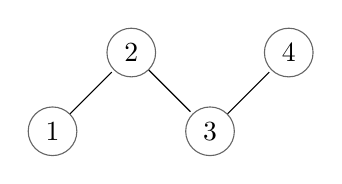
\begin{tikzpicture}[shorten >=1pt,->]
	\tikzstyle{vertex}=[circle, draw=black!60, minimum size=12pt]
	\node[vertex] (G_1) at (-1,-1) {1};
	\node[vertex] (G_2) at (0,0)   {2};
	\node[vertex] (G_3) at (1,-1)  {3};
	\node[vertex] (G_4) at (2,0)  {4};
	\draw [-] (G_1) -- (G_2);
	\draw [-] (G_2) -- (G_3);
	\draw [-] (G_3) -- (G_4);
	\end{tikzpicture}
\end{center}



\begin{center}
	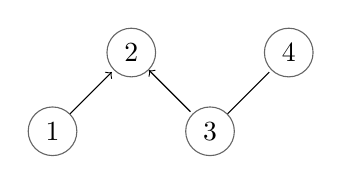
\begin{tikzpicture}[shorten >=1pt,->]
	\tikzstyle{vertex}=[circle, draw=black!60, minimum size=12pt]
	\node[vertex] (G_1) at (-1,-1) {1};
	\node[vertex] (G_2) at (0,0)   {2};
	\node[vertex] (G_3) at (1,-1)  {3};
	\node[vertex] (G_4) at (2,0)  {4};
	\draw [->] (G_1) -- (G_2);
	\draw [<-] (G_2) -- (G_3);
	\draw [-] (G_3) -- (G_4);
	\end{tikzpicture}
	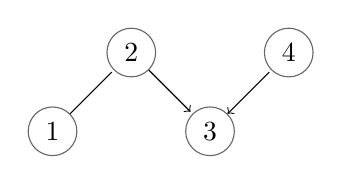
\begin{tikzpicture}[shorten >=1pt,->]
	\tikzstyle{vertex}=[circle, draw=black!60, minimum size=12pt]
	\node[vertex] (G_1) at (-1,-1) {1};
	\node[vertex] (G_2) at (0,0)   {2};
	\node[vertex] (G_3) at (1,-1)  {3};
	\node[vertex] (G_4) at (2,0)  {4};
	\draw [-] (G_1) -- (G_2);
	\draw [->] (G_2) -- (G_3);
	\draw [<-] (G_3) -- (G_4);
	\end{tikzpicture}
\end{center}

Figure - shows two possible orientations, depending on which v structure is oriented first, in the first case when we arrive at the 2,3,4 triple one of two thing can be done. The edge (3,4) can be left undirected or the new structure can override the old one, as shown in figure - .

\begin{center}
	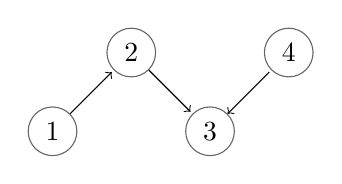
\begin{tikzpicture}[shorten >=1pt,->]
	\tikzstyle{vertex}=[circle, draw=black!60, minimum size=12pt]
	\node[vertex] (G_1) at (-1,-1) {1};
	\node[vertex] (G_2) at (0,0)   {2};
	\node[vertex] (G_3) at (1,-1)  {3};
	\node[vertex] (G_4) at (2,0)  {4};
	\draw [->] (G_1) -- (G_2);
	\draw [->] (G_2) -- (G_3);
	\draw [<-] (G_3) -- (G_4);
	\end{tikzpicture}
\end{center}

In the prexisiting R implementation the second approach of overwriting edges was taken so the same was done in the python implementation.

Finally the other orientatian rules described in the algorithm were followed, these were easy to implement using the networkx graphs as they consisted of testing for undirected and directed edges, then orienting based on those tests. This was repeated until no more edges were oriented, this completed the algorithm

\subsection{FCI Algorithm}

The FCI algorithm was able to use exactly the same code and first round v-structure orientation of the pc algorithm. However after this code unique to the fci algorithm must be developed.

First the final skeleton of the graph must be found. This is done by performing more independence tests, conditioned on the possible d-separating sets of the variables. Finding these sets was made simple by a networkx function to find paths between nodes on a graph.

For the rest of the algorithm the network is a PAG. The data structure used for the PAG was a subclass of the networkx undirected graph. In this graph the direction of an edge was determined by tags stored in a dictionary associated with that edge. This allowed all edge types of a PAG to be stored. 




\subsection{Testing}

To ensure that the algorithm was behaving as intended all parts must be thoroughly tested. The python unittest module was used to create a test suite covering as many aspects of the algorithm as possible.

For the chi squared independence test a sanity check consisting of testing whether a variable was independent of itself was used. Obviously the test will result in a p-value of 0 so was very easy to to test. This test was repeated in the case of a conditioning set of size 1 and size 2 to ensure this did not affect functionality.

Next a pre-existing test from r was used to find results on real data. This data was tested with the python implementation and the results compared. Data from the alarm\_10000 and the asia\_1000 datasets were used. Many tests with different variables and conditioning sets were performed.

To test the skeleton estimation again the R implementation was used. However, the R version does not use a chi squared test, a wrapper needed to be written to make it compatible with the R skeleton function. With this, skeletons could be generated from data in the same way in python and R and the results compared. The separation sets were also recorded and compared.

Testing the edge orientation for the PC algorithm first started with small sanity checks. For example the collider orientation was tested on networks with 3 nodes and two edges and simple separation sets.

The path checking needed for the pc algorithm was also  tested on small networks where paths were linear and some with many branches. It was also tested on a few negative examples.

Finally a skeleton and separation set generated from the alarms data was oriented in both R and python to test the whole edge orientation process as a whole. However due to the order dependence of the edge orientation the implementations produced slightly different results for the same graphs.

This meant that to test the edge orientation section of the pc algorithm, graphs had to be manually oriented using the algorithm and then compared to those estimated by the software.

For the FCI algorithm, the first part of the skeleton estimation is the same as in the PC algorithm  which is confirmed to function correctly. However, the final skeleton estimation needs to be tested so comparison testing was done with the R implementation.

Comparison of the edge orientation was performed, however due to the number of edge orientation rules it is likely that only some of them would be applied in a particular run. This means that to fully test  the rules they should be tested individually. So the rules were tested on graphs which should be oriented by the rule and that shouldn't be oriented by the rule. The graphs were then tested after rule had been applied to see if the rule functioned correctly.


\subsection{Final Structure}
The final implementation consisted of four main components. The$\chi^2$ test for independence, the skeleton estimation, PC edge orientation, and FCI edge orientation.

\subsection{Independence Test}
The $\chi^2$ test was a stand-alone function that can take a data frame along with the names of variables to be tested and a conditioning set. it returns a the $\chi^2$ statistic and a p-value from the test. The p-value represents the probability that the variables are not dependent conditioned on the conditioning set, if this statistic is high enough the variables can be considered independent.

\subsection{Graph Learners}
Each algorithm is implemented as a class, the base class of all algorithms is the graph leaner class. These class takes data and an independence test and learn a graph.

The base class implements the skeleton learning that all the algorithms use. It can also find and orient colliders on that skeleton. Finally, it has a static method to prepare data, this reads data from a file into a dataframe which can be used by the other methods.

The PC algorithm and the FCI algorithms were implemented as subclasses of the Graph learner. The PC algorithm only needed to implement the edge orientation step to complete the algorithm.

The FCI algorithm had to both implement edge orientation and extend the skeleton estimation of the graph learner.


\subsection{Graphs}  
Two new graph classes were implemented, the PDAG and the PAG. The PDAG is a fairly simple extension of networkx's built in Directed graph class in which undirected edges are merely stored as bidirected edges, in PDAGS there are no bidirected edges so ther will be no confusions between bidirected and undirected edges.

This implementation is simple but fairly powerful. Most built in networkkx functions will work in a reasonable manner. For example, the has\_edge function will be direction dependent on directed edges but not on undirected edges. Path finding algorithms will also work assuming undirected edges can be traversed in either direction.

\begin{center}
	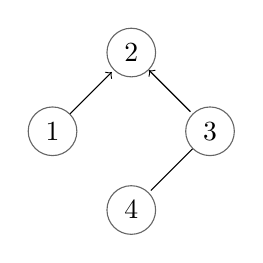
\begin{tikzpicture}[shorten >=1pt,->]
	\tikzstyle{vertex}=[circle, draw=black!60, minimum size=12pt]
	\node[vertex] (G_1) at (-1,-1) {1};
	\node[vertex] (G_2) at (0,0)   {2};
	\node[vertex] (G_3) at (1,-1)  {3};
	\node[vertex] (G_4) at (0,-2)  {4};
	\draw [->] (G_1) -- (G_2);
	\draw [<-] (G_2) -- (G_3);
	\draw [-] (G_3) -- (G_4);
	\end{tikzpicture}
	\quad\quad
	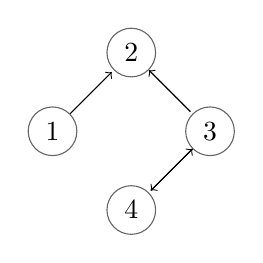
\begin{tikzpicture}[shorten >=1pt,->]
	\tikzstyle{vertex}=[circle, draw=black!60, minimum size=12pt]
	\node[vertex] (G_1) at (-1,-1) {1};
	\node[vertex] (G_2) at (0,0)   {2};
	\node[vertex] (G_3) at (1,-1)  {3};
	\node[vertex] (G_4) at (0,-2)  {4};
	\draw [->] (G_1) -- (G_2);
	\draw [<-] (G_2) -- (G_3);
	\draw [<-] (G_3) -- (G_4);
	\draw [->] (G_3) -- (G_4);
	\end{tikzpicture}
\end{center}

The PAG was more complex to implement due to the increased complexity of the graph. The PAG class is an extension of the undirected graph from networkx. All information about the tags, and therefore the directionality of the edges is stored in an attribute associated with particular edge. The attribute is a dictionary with keys being the nodes at each end of the edge and the values being the tag at that end of the edge.

This implementation meant that mayn new methods needed to be added and many existing methods modified. For example, when adding a new edge the tags of the edge needed to be assigned. methods for testing if edges were directed from u to v (had an arrow head into v) or fully directed from u to v (tail at u, arrowhead at v) were created and used during the FCI algorithm.

The built in methods for finding paths did however still work with this implementation which was very useful for edge orientation.

Currently viewing the graph as a whole is tricky, the built in functions for displaying graphs can not display the edge tags. It may be possible to use the display edge labels function to show the tags as a label on the graph.

\begin{center}
	\begin{tikzpicture}[shorten >=1pt,->]
	\tikzstyle{vertex}=[circle, draw=black!60, minimum size=12pt]
	\node[vertex] (G_1) at (-1,-1) {1};
	\node[vertex] (G_2) at (1,1)   {2};
	\node[vertex] (G_3) at (3,-1)  {3};
	\node[vertex] (G_4) at (1,-3)  {4};
	\draw [o->] (G_1) -- (G_2);
	\draw [<-] (G_2) -- (G_3);
	\draw [o-o] (G_3) -- (G_4);
	\end{tikzpicture}
\end{center}
\begin{center}	
	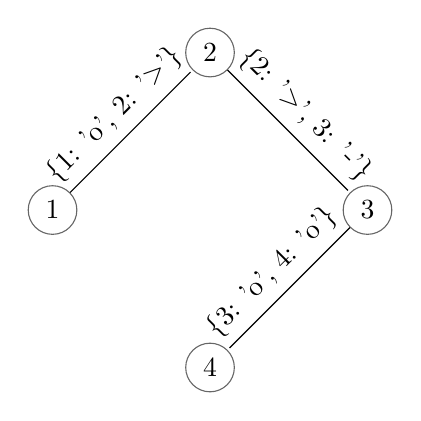
\begin{tikzpicture}[shorten >=1pt,->]
	\tikzstyle{vertex}=[circle, draw=black!60, minimum size=12pt]
	\node[vertex] (G_1) at (-1,-1) {1};
	\node[vertex] (G_2) at (1,1)   {2};
	\node[vertex] (G_3) at (3,-1)  {3};
	\node[vertex] (G_4) at (1,-3)  {4};
	\draw [-] (G_1) -- node[sloped, above]{\{1: 'o', 2: '$>$'\}} (G_2) ;
	\draw [-] (G_2) -- node[sloped, above]{\{2: '$>$', 3: '-'\}} (G_3);
	\draw [-] (G_3) -- node[sloped, above]{\{3: 'o', 4: 'o'\}} (G_4);
	\end{tikzpicture}
\end{center}
\section{Usage}
There are currently two main ways to use the python implementation, as a library and as a command line interface.

\section{Viewing Graphs}
There are a number of options to view a learned graph. Built in functions of the parent classes allow the edges and nodes to be iterated over to see where causal links have been estimated.

Options to view the graphs as adjacency matrices have also been implemented. In these matrices the rows represent the from node and the columns represent a to node. The order of the rows and columns is the same as the order in which the nodes are iterated over. The matrix is stored as a numpy array so it can be used with effiecient numpy methods in the future.

In the PDAG when there is a directed edge from one node to another there is a 1 in the appropriate position. If there is not a directed edge there is a zero. Directed edges going in both directions between nodes represent an undirected edge.
 
The PAG uses numbers greater than zero to represent the tags on an edge and zeroes to represent the absence of an edge. the '0' tag is represented as a 1, the '-' tag as a two and the '>' tag as a 3.

These matrices can also be written to files for future use. Each row of the matrix is written as a row and each point is separated by a space. The first row of the file consists of the to node name of the respective column and the first value of each row of points is the from node name. Examples for the PDAG in Figure \_ and the PAG in figure  \_ are shown in.  This representation can easily be used with a number of libraries including pandas, it can also be easily loaded into an R environment as a dataset.
\chapter{Analysis}
Analysis of this project will mainly consist of comparison to th implementation fo the algorithms in R. It will compare the functionality of the algorithms on data and also the run speed of the code.

\section{Initial Skeleton Generation}
The skeleton generation code has almost identical functionality as the R implementation. Even the order in which edges are tested is the same. However the R implementation has a non-order dependent mode which is not currently implemented in the python version however could be added as an option in the future.

The Alarm\_1000, Asia\_1000, and Diabetes\_1000 datasets found in  all produce identical skeletons as seen in Figure \_.

The $\chi^2$ test for independence was not implemented in the pcalg library in R. Other independence test for discrete data, such ad the $G^2$ test, were implemented. However, the bnlearn library has an implementation of the $\chi^2$ test to use for comparison.

Both tests return identical results on all tested data as seen in

\section{PC Algorithm Edge Orientation}
\begin{center}
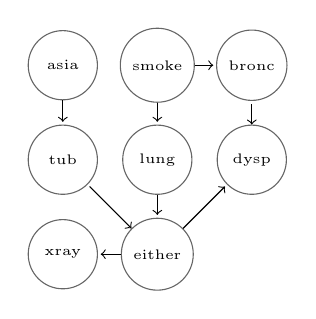
\begin{tikzpicture}[shorten >=1pt,->]
\tikzstyle{vertex}=[circle, draw=black!60, minimum size=25pt, font=\tiny]
\node[vertex] (asia) at (-1.2,1.2) {asia};
\node[vertex] (tub) at (-1.2,0) {tub};
\node[vertex] (smoke) at (0,1.2) {smoke};
\node[vertex] (lung) at (0,0) {lung};
\node[vertex] (bronc) at (1.2,1.2) {bronc};
\node[vertex] (either) at (0,-1.2) {either};
\node[vertex] (xray) at (-1.2,-1.2) {xray};
\node[vertex] (dysp) at (1.2,0) {dysp};
\draw [<-] (dysp) -- (bronc);
\draw [->] (smoke) -- (bronc);
\draw [->] (smoke) -- (lung);
\draw [->] (asia) -- (tub);
\draw [->] (lung) -- (either);
\draw [<-] (either) -- (tub);
\draw [->] (either) -- (xray);
\draw [->] (either) -- (dysp);

\end{tikzpicture}
\end{center}
\begin{center}
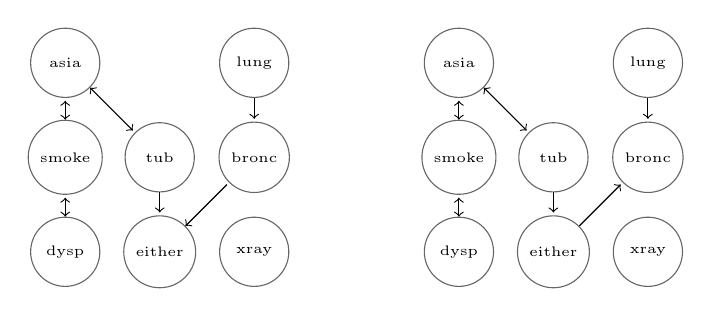
\begin{tikzpicture}[shorten >=1pt,->]
\tikzstyle{vertex}=[circle, draw=black!60, minimum size=25pt, font=\tiny]
\node[vertex] (asia) at (-1.2,1.2) {asia};
\node[vertex] (tub) at (0,0) {tub};
\node[vertex] (smoke) at (-1.2,0) {smoke};
\node[vertex] (lung) at (1.2,1.2) {lung};
\node[vertex] (bronc) at (1.2,0) {bronc};
\node[vertex] (either) at (0,-1.2) {either};
\node[vertex] (xray) at (1.2,-1.2) {xray};
\node[vertex] (dysp) at (-1.2,-1.2) {dysp};
\draw [<->] (dysp) -- (smoke);
\draw [<->] (smoke) -- (asia);
\draw [<->] (asia) -- (tub);
\draw [->] (tub) -- (either);
\draw [<-] (either) -- (bronc);
\draw [->] (lung) -- (bronc);[shorten >=1pt,->]

\node[vertex] (asia) at (3.8,1.2) {asia};
\node[vertex] (tub) at (5,0) {tub};
\node[vertex] (smoke) at (3.8,0) {smoke};
\node[vertex] (lung) at (6.2,1.2) {lung};
\node[vertex] (bronc) at (6.2,0) {bronc};
\node[vertex] (either) at (5,-1.2) {either};
\node[vertex] (xray) at (6.2,-1.2) {xray};
\node[vertex] (dysp) at (3.8,-1.2) {dysp};
\draw [<->] (dysp) -- (smoke);
\draw [<->] (smoke) -- (asia);
\draw [<->] (asia) -- (tub);
\draw [->] (tub) -- (either);
\draw [->] (either) -- (bronc);
\draw [->] (lung) -- (bronc);
\end{tikzpicture}
\end{center}

There are some differences in the edge orientation of the different implementations. For example, in the orient of asia\_1000 network, the edge either-bronc is oriented in opposite directions by the two implementations. When tested on other datasets very similar results were found, with identical skeletons but occasional slight differences in edge orientation due to the order in which colliders are oriented. This is due to the order in which the colliders were oriented in the graph. In the R implementation the triple lung, bronc, either is oriented followed by the triple tub, either bronc. This causes the edge either-bronc to be overwritten and reoriented. In the python implementation this is done in the opposite order resulting in a different network.

Neither order is more correct than the other however this orientation is used in the FCI algorithm so differences in the order can have a  knock on effect in the PAGs estimated by this algorithm.

Both estimates are quite different from the actual network which generated the data.

\section{FCI Algorithm Final Skeleton}
The FCI algorithm begins with the skeleton estimation and collider orientation to that of the PC algorithm. However because an edge in a PDAG can be bidirectional the order of of collider orientation will have no effect on the final structure of the skeleton.

To estimate the final skeleton the possible-d-sep sets must be found for every node in the graph. The implementations however find slightly different possible-d-sep sets for the same graph. The R implementation appears to be using a slightly different method to find these sets. This can be illustrated with the asia\_1000 dataset.

Figure \_ shows the skeleton of the graph when the possible-d-separation sets are found, this is the same in both implementations. However the sets found for the tub node and the smoke node are not equal. The R implementation does not add the smoke node to the possible-d-separation set of tub despite the the node between them being a collider. This does not affect the estimation of this particular graph, however it will affect other graphs and since it is done fairly early on in the algorithm it can have large knock-on affects on the end result.

\section{FCI Algorithm Edge Orientation}

\section{Run Speed}
The cProfiling library was used to collect statistics about the implementation. The library collects the number of times each function is called by the code along with the execution time of the code. This profiling allows the bottle necks of the code to be found and made high priorities or optimisation.

The independence test was the main bottleneck of the algorithms, and was significantly slower than the R implementation. This is because the R implementation actually runs C code behind the scenes, C code is compiled rather than interpreted like python and R. This makes the code much faster.

Calculating the contingency tables was the most expensive part of the independence test. Currently it uses a built in function from the pandas library. Replacing this function with something faster could make a large difference to the run speed.

However, the independence test in the algorithm is a parameter and thus the current slow test could be wholly replaced by a faster version. This new test could call C code like the R implementation.

\chapter{Conclusion}
\section{Further Work}
The most obvious extension to this project would be to implement the RFCI algorithm described in the literature review. Due to time constraints it was not implemented for this project. However the PAG class implements the majority of functionality needed to implement the RFCI algorithm. The process of implementation would be very similar to the process of implementing the FCI algorithm.

Another improvement would be to increase the speed of the conditional independence tests. One approach could be to implement the independence test in C and interface with it using Cython. C programs are much faster than those written in python so there would almost definitely be an improvement.

Other independence tests could also be written. These tests could be for the same kind of data as the $\chi^2$ or it could be a test for other data for example continuous data. The raw data would not even be necessary input to the algorithm, instead some sufficient statistics placed in a pandas data frame could be used if the independence test was able to estimate independence based on these statistics.

\appendix
\chapter{Some apendix}
\printbibliography
\end{document}